\chapter{Bitcoin, a peer-to-peer payment network}
\label{chap:bitcoin}

The Bitcoin ecosystem is composed of multiple actors. Users of the network access
information via wallets in their laptop or mobile phone. These users can see the amount
present in their addresses. An address is the representation of a public key, herself
being the representation of a private key. An address is owned by a user if this user
has in his possession the associated private key. Users can transfer funds from some
of their addresses to other addresses owned by other users or theirself. When funds
are transfered a transaction is created and send to the network. The network is
composed by nodes and these nodes take care of its proper functioning. Some of these
nodes are called miners, they listen to new transactions and try to include them into
the blockchain. This blockchain is the output, the intrinsec result, of the Bitcoin
protocol and can be compared to a distributed public ledger. Nodes are softwares
running all over the world, these softwares are maintained and improved by a group
of developers present all over the world and for Bitcoin, the original and reference
implementation is Bitcoin-core. The software allows to interact with the blockchain.
It is possible to retreive information such as current unconfirmed transactions,
information present in the blockchain, amount available for an address, etc.
An unconfirmed transaction is a transaction that has not been yet included into
the blockchain.

In the following some building blocks needed to figure out how payment channels works
and how we can improve them with some cryptography are traveled. If you are a master
of Bitcoin and you already know how blocks are created, how transactions are structured,
how fees are calculated and how segregated witness works, this chapter will be just
a reminder. For further explaination the best ressource today is the book \say{Mastering
Bitcoin} by Andreas Antonopoulos \cite{Antonopoulos:2014:MBU:2695500}.

% type of nodes in the peer-to-peer network
% \url{https://github.com/bitcoinbook/bitcoinbook/blob/second_edition/ch08.asciidoc}

\minitoc

\newpage

% -----------------------------------------------------------------------------
\section{The blockchain}

The blockchain, as indicated by his name, is a chain of blocks. Blocks are created
by the miners in a race to find the next valid block called the mining process. A block is considered valid
if its identifier, i.e. the double hash of its header, is lower to the current
difficulty target. It is worth noting that the validity of a block is based on multiple
other criterion who are not exposed here, for further information please refer
to the book \say{Mastering Bitcoin}. The header of a block is composed of a version
number, a creation timestamp, a nonce, or the difficulty target used as boundary.

The difficulty target is adjusted so a valid block is found in the network every
ten minutes in average. Mining can be modelized as a poisson process, i.e. the probability
of a given number of events occurring in a fixed interval of time or space if these
events occur with a known constant rate is independent of the time since the last event.
A miner will create a candidate block and compute its identifier, if this identifier
is lower than the current difficulty target then the block is valid and the miner notice
the network that he found the next block. Then the process start again. If the block
identifier is not valid the miner can change the nonce value in the header and
check with the new identifier. Finding the next valid block is so a computation that
require an enormous amount of power. All the network, round the clock, keeps searching
for the next valid block and the power of computation increase day after days.

\subsection{A chain of blocks}

As mentioned before, the blockchain is a chain who must be secure, verifiable,
and immutable. To achieve immutability, modification of previous blocks must
invalidate the chain. The block identifier is affected by information like the
creation timestamp or the nonce used to adapt the modifier but also from the
previous block identifier in the chain. That means that if the previous block
identifier is changed for exemple, because its content changed, the child block
into the chain will become invalid as well as its child, and so on.

Modifying the blockchain without invalidate the chain require to recompute all the
block identifiers after the changed block. This require a quantity of power that
can be estimated and for which the costs represent a certain safety threshold.
It is established that a transaction included in a block can be considered as safe
after six child blocks. The amount of power needed to erase this transaction became
statistically too high to be probable, but it does not means that it will never happen
due to the fact that there is the same probability to find a valid block with the
first nonce than with the thousandth.

\subsection{A list of transactions}

To be useful, a block needs a content. In Bitcoin the content of a block is composed
of transactions. As mentioned before, a transaction is called \textit{confirmed} when
she is included in a block. The number of confirmation is related to the number of
blocks mined after that the transaction has been included.

To keep track of all the transactions included into a block, a Merkle tree is created.
A Merkle tree or hash tree is a is a tree in which every leaf node is labelled with
the hash of a data block and every non-leaf node is labelled with the cryptographic
hash of the labels of its child nodes.

\begin{figure}[H]
	\centering
	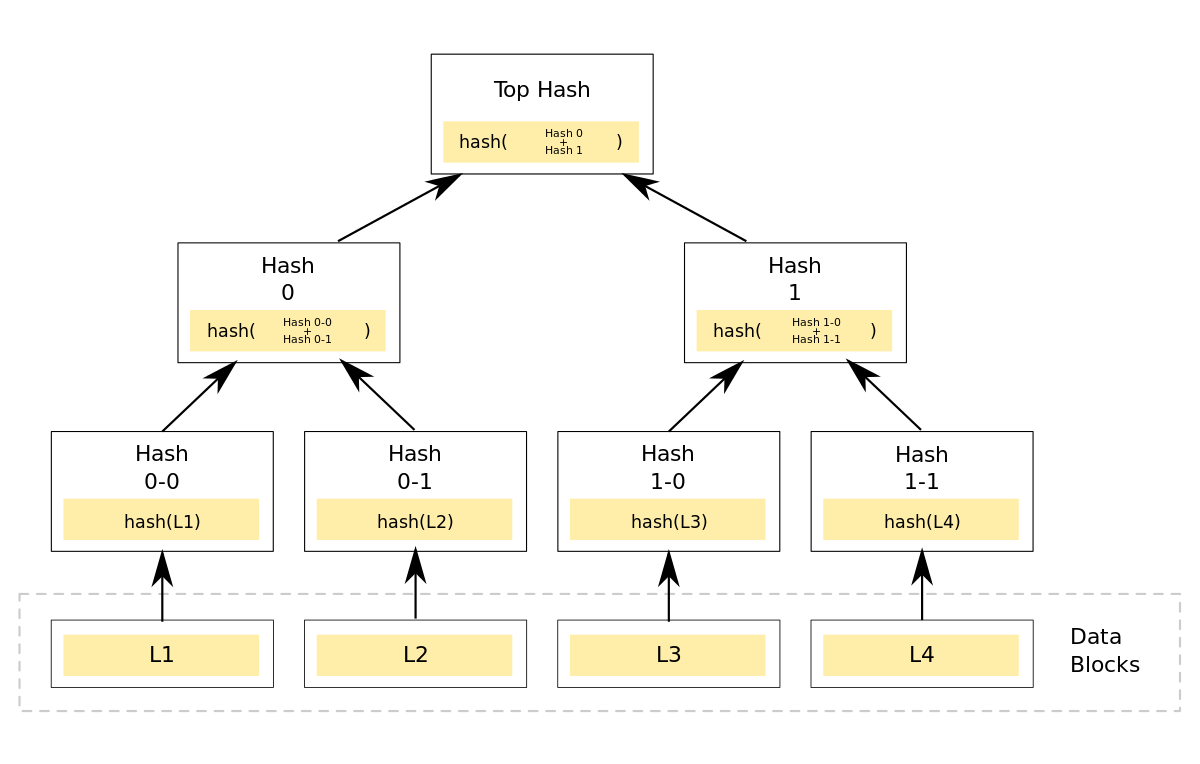
\includegraphics[width=1\columnwidth]{merkleTree}
	\captionsource{Merkle tree construction}{Merkle tree construction}
	{\url{https://en.wikipedia.org/wiki/Merkle_tree}}
	\label{fig:merkleTree}
\end{figure}

Given the top hash or Merkle root and a leaf, it is possible to prove the membership
by given the path for each complementary hashes. E.g given the Merkle root and \texttt{L1},
the proof is \texttt{Hash 0-1} and \texttt{Hash 1}. The verifier can then compute
the hash of \texttt{L1}, the result of this hash with \texttt{Hash 0-1}, and then with
\texttt{Hash 1}. If the result is the same as the Merkle root, then \texttt{L1} is a part
of the tree.

In a block, a Merkle tree of all included transaction identifiers is created. The
obtained Merkle root is put into the header of the block. To validate if a transaction
is included in a block the path must be given, then the resulting hash is compared
to the Merkle root registered in the block's header.

% -----------------------------------------------------------------------------
\section{Transactions}

Transactions allow users to move Bitcoins from an address to another and they create
the content of the Bitcoin's blockchain. In Bitcoin, the blockchain does not store a
balance for each user, the blockchain keeps only the history of all transactions that
have been made since the begining.

\subsection{A list of inputs \& outputs}

A transaction is composed of a list of inputs and a list of outputs. In other words,
where the Bitcoins come from and where they go. An input refers to an address where
the funds will be spend, and an output refers to an address where the funds will
go. An input points to another transaction output who has not been used already.
Inputs and outputs are links, to spend funds the user need to control addresses
where unspend outputs are present. These unspend outputs are called \texttt{UTXOs}
and represent the total amount own by a user.

\begin{figure}[H]
	\centering
	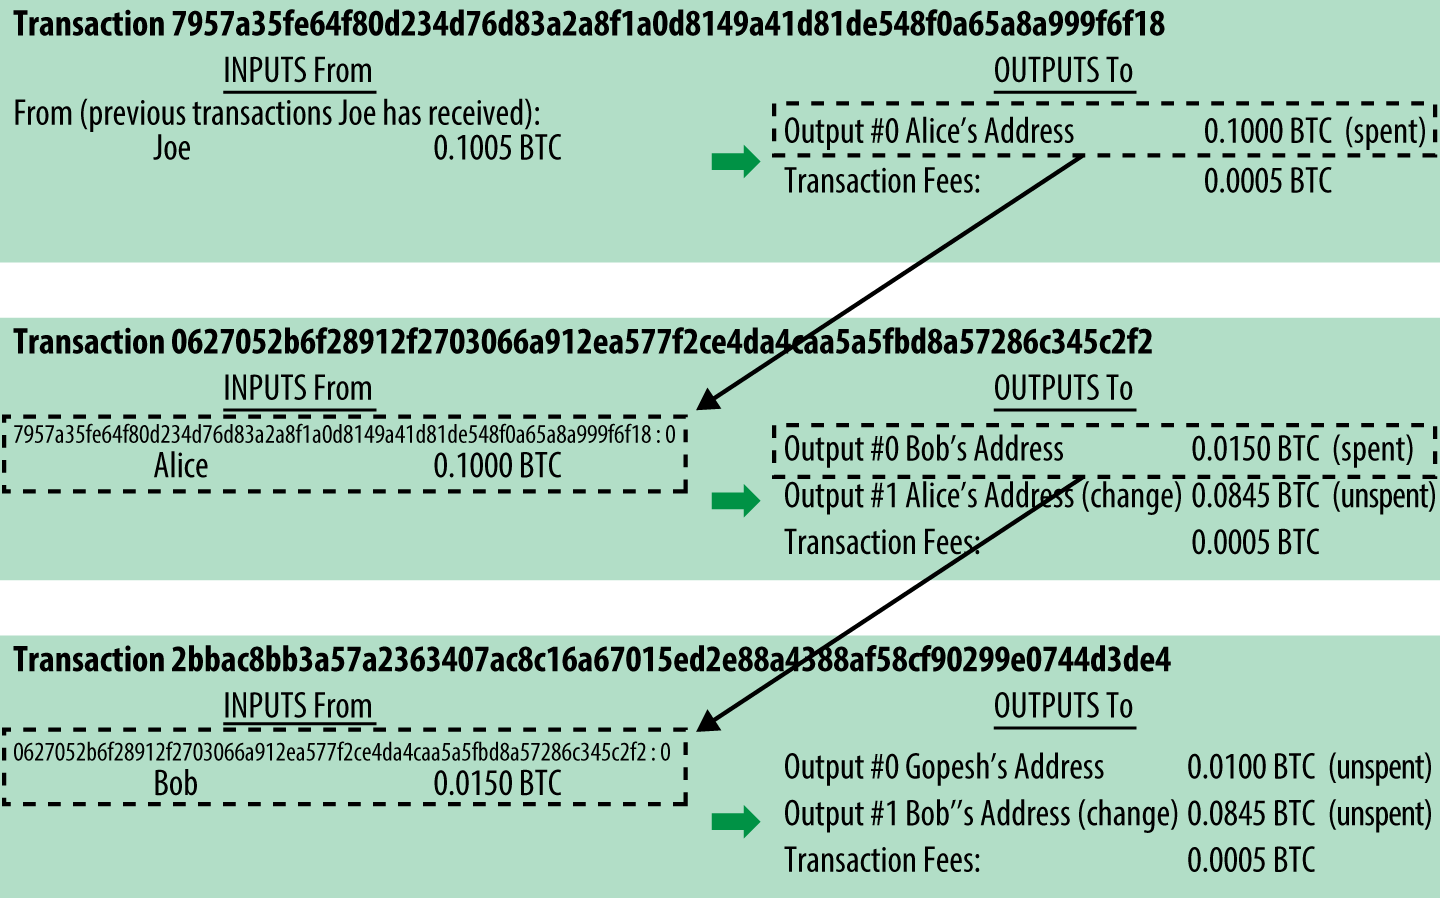
\includegraphics[width=1\columnwidth]{utxosChain}
	\captionsource{A chain of transactions where inputs and outputs are linked}
  {A chain of transactions where inputs and outputs are linked}
	{\url{https://github.com/bitcoinbook/bitcoinbook/blob/second_edition/ch02.asciidoc}}
	\label{fig:utxosChain}
\end{figure}

Each input is attached to a value (the value specified in the output to which the
input points). The sum of all inputs in a transaction must correspond to the sum
of all the values specified in the outputs, as in a dual entry accounting. So an
input must be spend entirely.

So, the most simple transaction is composed of one input and one output with the same
amount of money in and out.
However, the most standard transaction is composed of one input, refering from where the
funds come from, and two outputs. Indeed, it is very rare to have the right amount
available in one \texttt{UTXO}. So, the first output is the user who will receive
the funds, with the amount transfered, and the second output is an other address
owned by the sender to gather the change, i.e. the remaining amount.

As blocks, transactions have identifier. These identifiers are created in the same
way as blocks, by taking the double hash of the data, i.e. the signed transaction.
That means that, in the original design, a transaction does not have its final
transaction identifier (TXID) before she is completely signed (every inputs).

\subsection{Transaction fees}

The sum of all inputs in a transaction must correspond to the sum of all the values
specified in the outputs, yes but if the sum of all outputs is lower than the sum
of the inputs, the difference is implicitly considered as a fee (as shown in
Figure~\ref{fig:utxosChain}.) At the beginning no fee was required, but today a
transaction will not be included in a block without paying fees. A miner, when he
find a block, can create a special transaction---the first transaction in the
block---without inputs, where a regulated amount of new coins is created plus the
total amount of fees collected in all the included transactions. A miner will therefore
select the transactions that pay the more fees in relation to the amount of work needed
to validate them. Fees are calculated in relation to the size of the transaction
in bytes, an ratio of fee per byte is then selected to find the fee for a transaction.

\subsection{Scripting language}

As described before, \texttt{UTXO}s, so outputs, are related to addresses and a proof
of ownership is required to spend an \texttt{UTXO}. To achieve this, the Bitcoin
protocol use digital signatures. To spend an \texttt{UTXO}, a valid signature for
to the address, and so the public key, is required and to sign a transaction the
private key is required. Thus, while signing a transaction corresponding to the
right address it is possible to prove that the user own the address. But the
protocol does not just require signatures and public keys, conditions to
\textit{unlock} an \texttt{UTXO} are structured in scripts. Bitcoin has a stack
based script language called \say{Bitcoin Script}.

\begin{figure}[H]
	\centering
	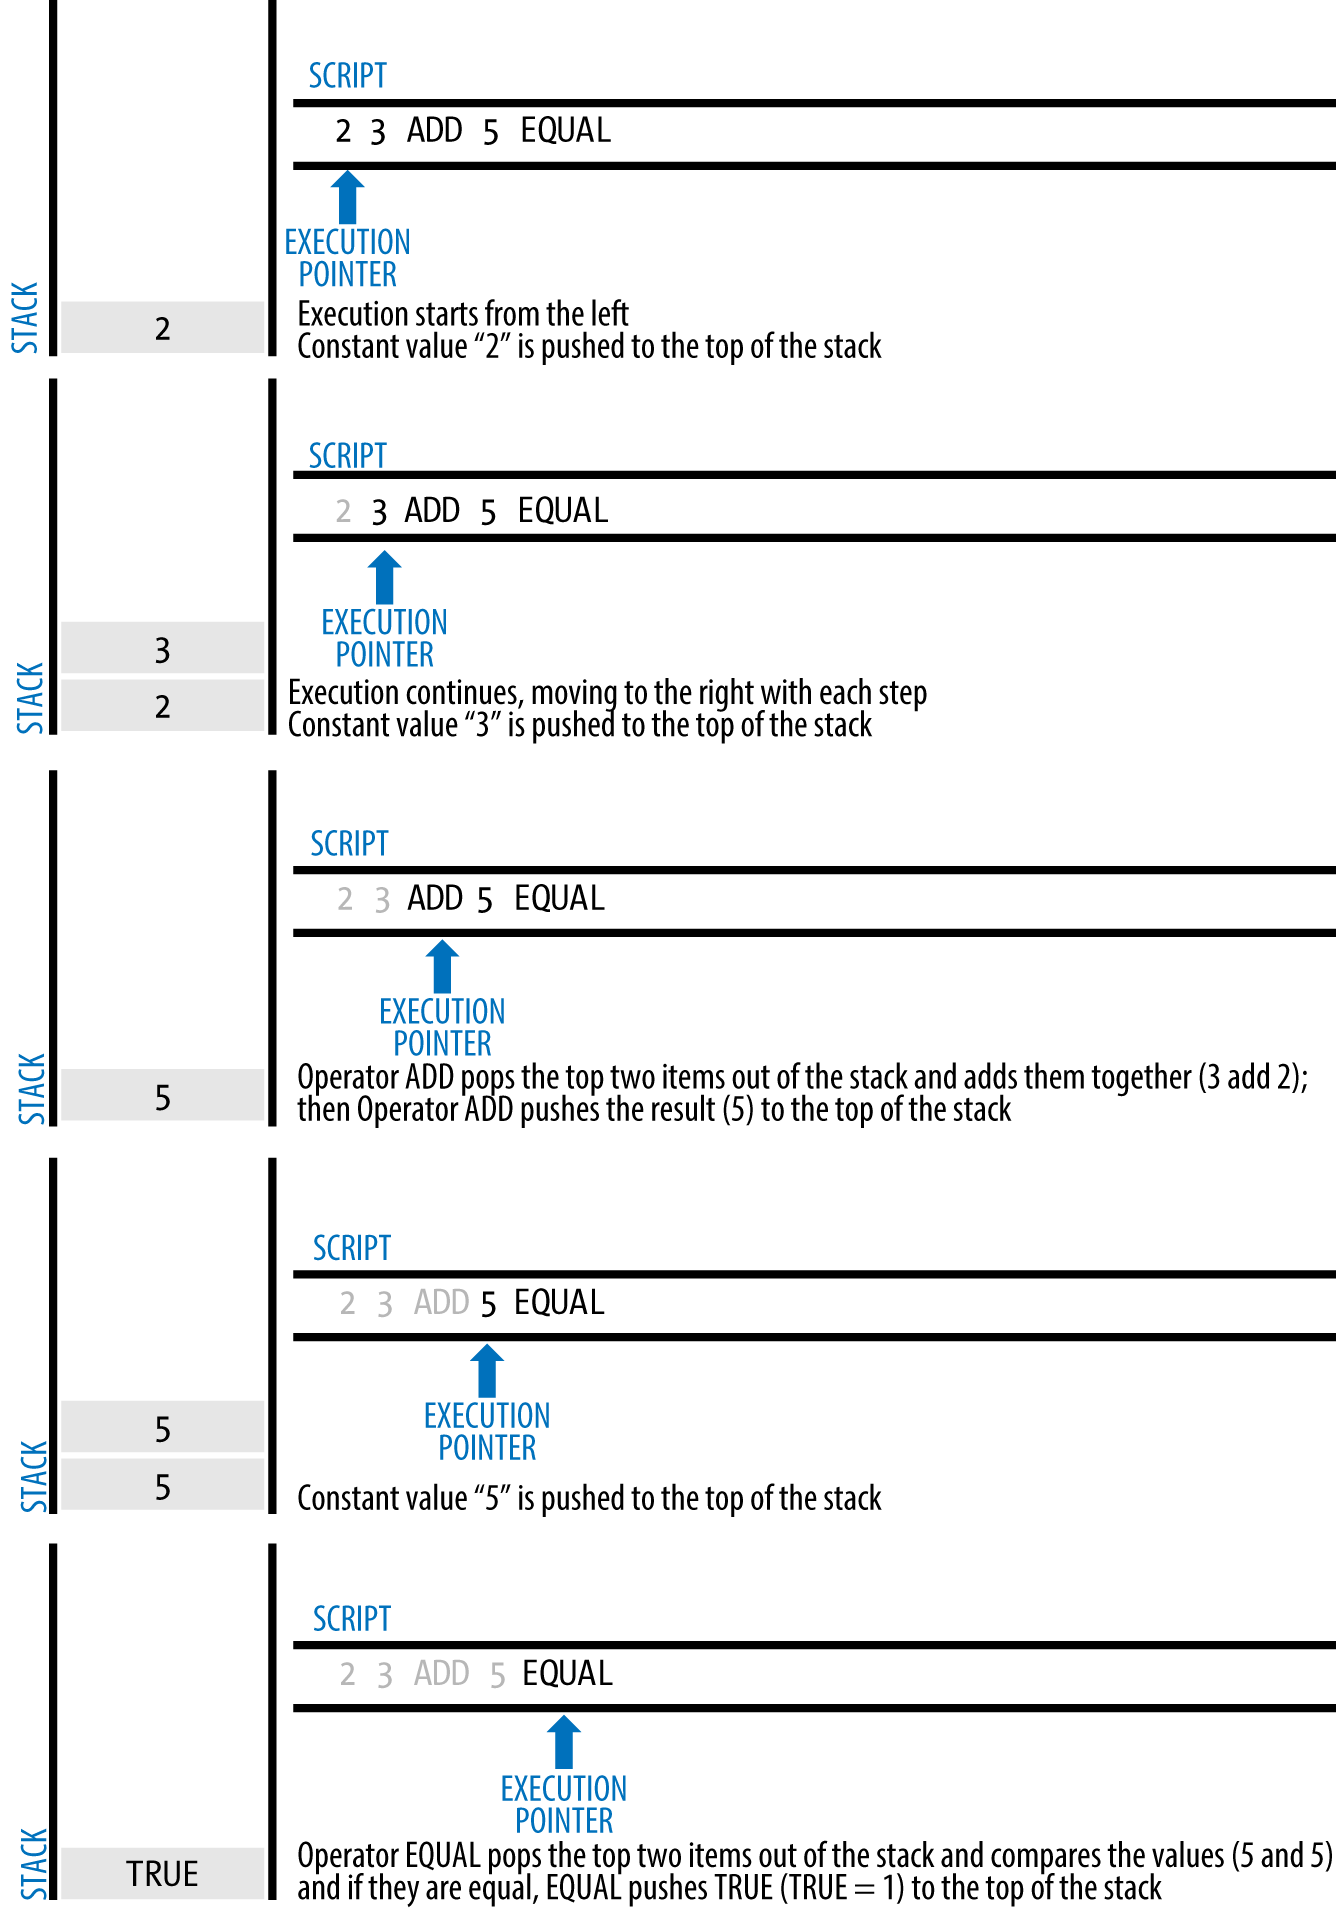
\includegraphics[width=0.73\columnwidth]{stackBased}
	\captionsource{Example of simple Bitcoin script program execution}
  {Example of simple Bitcoin script program execution}
	{\url{https://github.com/bitcoinbook/bitcoinbook/blob/second_edition/ch06.asciidoc}}
	\label{fig:stackBased}
\end{figure}

The list of all the \texttt{OP\_CODES} available in the Bitcoin script language is
in the documentation. Among them, \texttt{OP\_CHECKSIG} to verify a signature given
a signature and a public key onto the stack, \texttt{OP\_IF, OP\_ELSE, OP\_ENDIF} to
create execution branch given a boolean onto the stack, \texttt{OP\_DUP} to duplicate
the value onto the stack, or \texttt{OP\_HASH160, OP\_SHA256} to compute hashes of
values onto the stack.

Each input and output have a script. For an output the script correspond to the
requirement to be fulfilled to be allowed to spend it. An address is the result of
the public key hashed with a \texttt{SHA256} and then hashed with a \texttt{RIPEMD160}
encoded with a checksum in a more human readable format. When an address is given,
a user can decode the human readable format to retreive the hash data and create
an output script called \gls{p2pkh}. With the script, the address can be retreived,
and given the address and the script, only the user who own the private key
corresponding will be able to sign the transaction and spend the funds. The user
owning the address can create a transaction such as an input points to the \texttt{UTXO}.
To unlock the funds, the user needs to sign the transaction and give the signature
with the public key in the input's unlocking script. A miner, before including a
transaction in a candidate block, validate all the inputs. He needs to check if the
pointed output is realy an \texttt{UTXO} and execute the locking script with the
unlocking script. To do so, both scripts are concatenated with the unlocking script
first and executed (as shown if Figure~\ref{fig:lockUnlock}).

\begin{figure}[H]
	\centering
	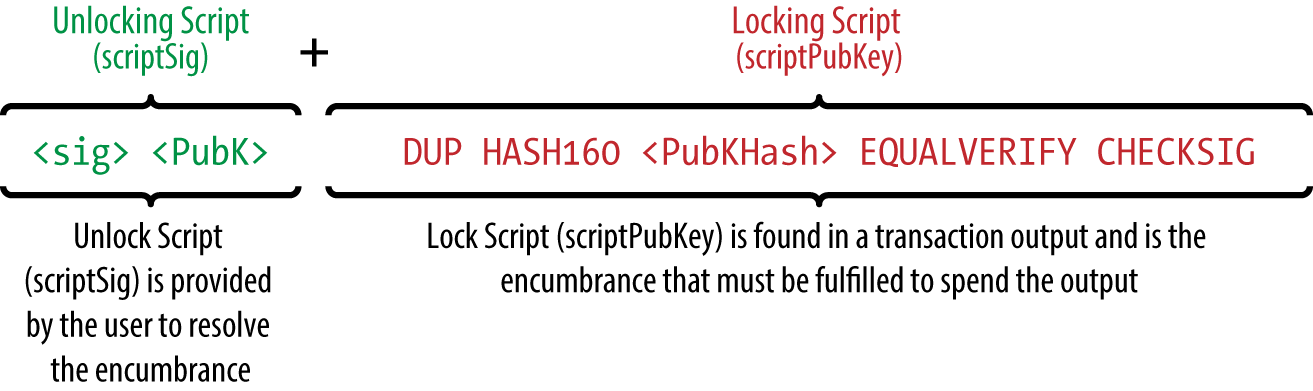
\includegraphics[width=1\columnwidth]{lockUnlock}
	\captionsource{Example of pay to public key hash script}
  {Example of pay to public key hash script}
	{\url{https://github.com/bitcoinbook/bitcoinbook/blob/second_edition/ch06.asciidoc}}
	\label{fig:lockUnlock}
\end{figure}

This script in Figure~\ref{fig:lockUnlock}, when executed, will put the signature
onto the stack, then the public key, the public key will be duplicate and the
public key ontop of the stack will be hashed, the public key hash present in the
locking script is put ontop of the stack and the two first element ontop of the
stack will be compare. If the comparison failed, the script will failed and the
transaction will be rejected as invalid. If the test pass, the signature will
be check with the two remaining parameter onto the stack, the public key and the
signature. If the signature is valid, the value \texttt{True} is put onto the
stack, otherwise the value \texttt{False} is put onto the stack. If the value
\texttt{True} is present onto the stack at the end of the script the transaction
is valid, otherwise the transaction is invalid.

\subsection{Segregated witness}

\gls{segwit} is the \gls{bip} 141 that propose to change the transaction structure
in order to fix transaction malleability, add script versionning, and improve other
aspects \cite{SegWit, SegWitBIP}. In fact, \gls{segwit} change the way outputs are
structured, the malleability is fixed only if all inputs use \gls{segwit}. A
transaction can have \gls{segwit} inputs and non-\gls{segwit} inputs at the same
time.

\begin{quote}
  This BIP defines a new structure called a \say{witness} that is committed to
  blocks separately from the transaction merkle tree. This structure contains
  data required to check transaction validity but not required to determine
  transaction effects. In particular, scripts and signatures are moved into this
  new structure.

  The witness is committed in a tree that is nested into the block's existing
  merkle root via the coinbase transaction for the purpose of making this BIP
  soft fork compatible. A future hard fork can place this tree in its own branch.
\end{quote}

With a \gls{segwit}, a transaction have two TXID. The first is determine without
all the witness data, so it is deterministic when the transaction is created,
before any signature. The second one is related to the witness data. This fix
the transaction malleability. The second big change is the way the size for the
fees are calculated. The transaction weight \texttt{Tx Weight} becomes
$\texttt{Base Tx} * 3 + \texttt{Total Size}$ where \texttt{BaseTx} is the size
without the witness data and \texttt{Total Size} is the serialized transaction
with all the data, including the witness data.
The fees are now calculated with the virtual transaction size such as virtual
size is equal to $\texttt{Tx Weight} / 4$. Thus, the weight of the witness data
in the calculus of the fees is reduced.

% -----------------------------------------------------------------------------
\section{Scalability of Bitcoin}

% -- Your text goes here --

\subsection{On-chain improvements}
\subsection{Layer-two applications}
